% Node Type Hierarchy Diagram
% Shows different node types and their capabilities
%
% ACCESSIBILITY ALT TEXT:
% A vertical hierarchy diagram showing three node types. Top: Minting Node
% (orange box) - block producer with PoW and SCP participation, requires
% 200+ GB storage and 16 GB RAM. Middle: Full Node (blue box) - validator
% with complete blockchain storage and transaction validation, requires 100+
% GB and 8 GB RAM. Bottom: Light Client (green box) - wallet with headers
% only and SPV proofs, requires minimal resources. Dashed arrows show
% inheritance (Full extends to Minting) and trust (Light trusts Full).
% Left brace indicates decreasing trust requirements from top to bottom.

\begin{figure}[ht]
\centering
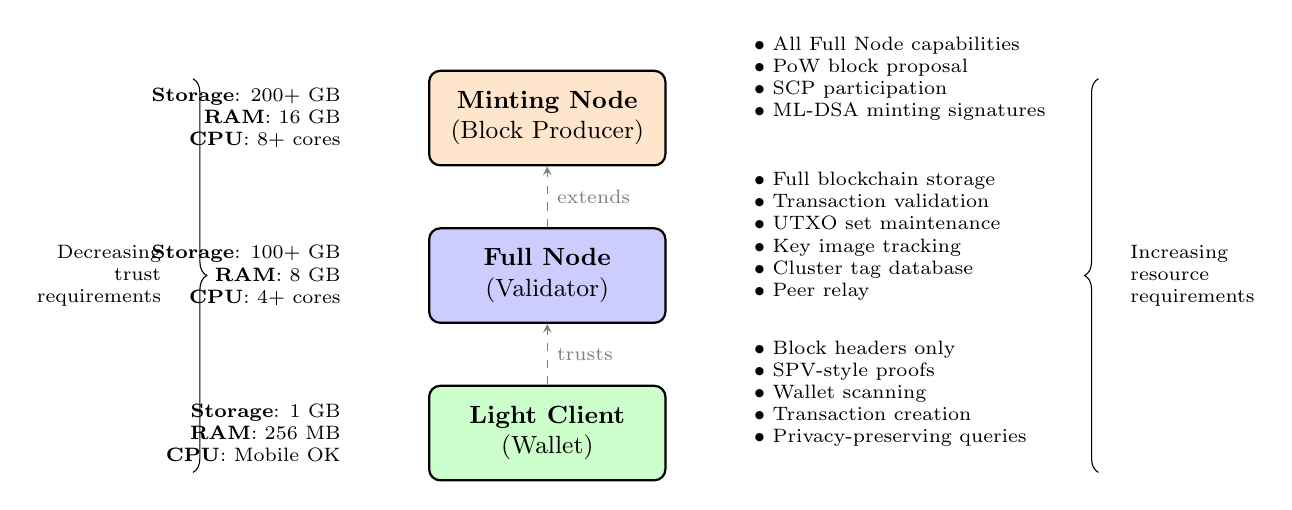
\begin{tikzpicture}[
    node distance=1cm,
    nodetype/.style={rectangle, draw, rounded corners, minimum width=3cm, minimum height=1.2cm, align=center, font=\small},
    full/.style={nodetype, fill=blue!20, thick},
    minting/.style={nodetype, fill=orange!20, thick},
    light/.style={nodetype, fill=green!20, thick},
    capability/.style={font=\scriptsize, align=left},
    arrow/.style={->, >=stealth, thick},
    inherit/.style={->, >=stealth, dashed, gray},
]

% Node types (arranged in hierarchy)
\node[minting] (minting) at (0,4) {\textbf{Minting Node}\\(Block Producer)};
\node[full] (full) at (0,2) {\textbf{Full Node}\\(Validator)};
\node[light] (light) at (0,0) {\textbf{Light Client}\\(Wallet)};

% Inheritance arrows
\draw[inherit] (full) -- (minting) node[midway, right, font=\scriptsize] {extends};
\draw[inherit] (light) -- (full) node[midway, right, font=\scriptsize] {trusts};

% Capabilities for Minting Node
\node[capability, anchor=west] at (2.5,4.5) {
    $\bullet$ All Full Node capabilities\\
    $\bullet$ PoW block proposal\\
    $\bullet$ SCP participation\\
    $\bullet$ ML-DSA minting signatures
};

% Capabilities for Full Node
\node[capability, anchor=west] at (2.5,2.5) {
    $\bullet$ Full blockchain storage\\
    $\bullet$ Transaction validation\\
    $\bullet$ UTXO set maintenance\\
    $\bullet$ Key image tracking\\
    $\bullet$ Cluster tag database\\
    $\bullet$ Peer relay
};

% Capabilities for Light Client
\node[capability, anchor=west] at (2.5,0.5) {
    $\bullet$ Block headers only\\
    $\bullet$ SPV-style proofs\\
    $\bullet$ Wallet scanning\\
    $\bullet$ Transaction creation\\
    $\bullet$ Privacy-preserving queries
};

% Storage requirements (left side)
\node[font=\scriptsize, anchor=east, align=right] at (-2.5,4) {
    \textbf{Storage}: 200+ GB\\
    \textbf{RAM}: 16 GB\\
    \textbf{CPU}: 8+ cores
};

\node[font=\scriptsize, anchor=east, align=right] at (-2.5,2) {
    \textbf{Storage}: 100+ GB\\
    \textbf{RAM}: 8 GB\\
    \textbf{CPU}: 4+ cores
};

\node[font=\scriptsize, anchor=east, align=right] at (-2.5,0) {
    \textbf{Storage}: 1 GB\\
    \textbf{RAM}: 256 MB\\
    \textbf{CPU}: Mobile OK
};

% Trust model annotation
\draw[decorate, decoration={brace, amplitude=5pt, mirror}]
    (-4.5,-0.5) -- (-4.5,4.5)
    node[midway, left=8pt, font=\scriptsize, align=right] {
        Decreasing\\
        trust\\
        requirements
    };

\draw[decorate, decoration={brace, amplitude=5pt}]
    (7,-0.5) -- (7,4.5)
    node[midway, right=8pt, font=\scriptsize, align=left] {
        Increasing\\
        resource\\
        requirements
    };

\end{tikzpicture}
\caption{Node type hierarchy in \Botho. Light clients trust full nodes for
transaction validation but verify headers independently. Full nodes maintain
complete state and validate all transactions. Minting nodes extend full nodes
with block proposal capabilities. Resource requirements scale with trust
assumptions---light clients trade some security for accessibility.}
\label{fig:node-hierarchy}
\end{figure}
